\subsection{Architektura aplikacji}
Jako model architektury aplikacji przyjęto architekturę wartstwową. Pozwala ona odseparować zadania wykonywane przez
poszczególne komponenty aplikacji, ułatwiając utrzymanie kodu. Jest to osiągane poprzez rozgranizczenie zadań
realizowanych przez poszczególne warstwy. Architektura wartstwowa charakteryzuje się hierarchicznym układem komponentów,
co przekłada się na zwiększenie przejrzystości pozwalające na elastyczny rozwój aplikacji.
W ramach projektu zastosowano trzy warstwy podziału:
\begin{itemize}
	\item Warstwa dostępu do danych — odpowiadająca za komunikacje z bazą przy użyciu modelu encji.
	\item Warstwa logiki biznesowej — obejmująca szczególnie serwisy zarządzania stanem aplikacji.
	\item Warstwa prezentacji — realizowana przez komponenty Vue.
\end{itemize}

<diagram architektury>

\subsection{Warstwa dostępu do danych}
\subsubsection{Modele bazodanowe}
Dane użytkownika, zapisywane w aplikacji można sklasyfikować jako forma \enquote{notatek}.
Zdecydowano się nadać im modułowy charakter, pozwalając w ten sposób na wykorzystywanie różnych typów notacji muzycznej
w ramach określonego zbioru, który sumarycznie może opisywać aranżowany utwór.
Wykorzystano stąd dwupoziomowy podział obiektów. Jako pierwszy poziom przyjęto koncepcję
\enquote{zeszytu do nut}, jako zbioru notatek,
co przynosi stosowną nazwę wykorzystaną w kodzie źródłowym \enquote{book} (od ang.
music book — \textit{zeszyt do nut}).

<encja zeszytu i opis pól>

Idąc dalej tym tokiem, przyjęto określenie \enquote{page} (z ang. — textit{strona}),
jako odnoszące się do poziomu drugiego — pojedynczej notatki użytkownika.

<encja książki i opis pól>

Obie encje implementują prosty interfejs Entity, deklarujący pole id,
ułatwiając działanie serwisów zarządzających persystencją:

<interfejs entity>

Jako wyznacznik powiązań między encjami Book i Page, w bazie przechowywana jest dotatkowo tablica obiektów Index.
Z uwagi na jej nadrzędny charakter, nie implementuje ona od interfejsu Entity. Występuje w bazie pojedynczo, pod ustalonym
kluczem \enquote{INDEX}.

<encja index>

\subsubsection{Serwisy zarządzające persystencją}
W aplikacji zastosowano bazę danych Ionic Storage. Jest to baza typu klucz-wartość. Aby umożliwić
zarządzanie obiektami zagnieżdżonymi — jako: \textit{zeszyt} zawierać może wiele \textit{stron} — przy zachowaniu
niezależności operacji na obiektach, zastosowano trzy serwisy:
\begin{itemize}
	\item StorageWrapper

	      Z uwagi na charakter kluczy i wartości bazy — jako dwóch ciągów znaków — obiekty zapisywane w bazie są
	      konwertowane do ciągów JSON. StorageWrapper \textit{Opakowuje} bibliotekę Ionic Storage, udostępniając podstawowe
	      metody zarządzania danymi oraz konwertując przetwarzane dane na ciągi znaków JSON i odwrotnie.
	      Jako jedyny bezpośrednio korzysta z metod oferowanych przez Ionic Storage.
	\item PersistencyService

	      Z StorageWrappera korzysta explicite PersistencyService, wykorzystujący jego metody w kontekście konkretnych obiektów.
	      Zawiera logikę opartą o interfejs Entity, implementowany przez encje Book i Page. Odwołuje się do danych
	      serwisu Indexer, celem identyfikacji i lokalizacji obiektów zapisanych w bazie.
	\item Indexer

	      Poza encjami Book i Page przechowywana jest również tablica obiektów Index określająca
	      zależności między encjami. Stąd stan początkowy Indexera jest wczytywany z bazy przez PersistencyService
	      na początku działania aplikacji.
	      Informacje o zmianach są sygnalizowane przez serwisy zarządzania stanem aplikacji.
	      Odpowiadając na nie, serwis Indexer zapewnia zgodność tablicy Indexów ze stanem rzeczywistym
	      \textit{biblioteki} użytkownika. W pewnym stopniu emuluje on możliwości bazy relacyjnej.
\end{itemize}

Zależności między opisanymi serwisami obrazuje przedstawiony poniżej diagram:

<diagram persystencji>

\subsection{Warstwa logiki biznesowej}
\subsubsection{Serwisy zarządzające stanem aplikacji}
Warstwę logiki biznesowej stanowią serwisy zarządzania stanem aplikacji.
Wszystkie opierają się na bibliotece Pinia.
Umożliwia to funkcjonowanie niezależne od komponentów Vue aplikacji, udostępniając dla nich globalny stan,
do którego mogą się odwoływać.

Aby rozdzielić zadania tej warstwy, serwisy zostały podzielone według domen:
\begin{itemize}
	\item LibraryService — odpowiada za zarządzanie biblioteką zeszytów użytkownika.
	\item TagService — udostępnia zbiór tagów utworzonych w ramach biblioteki użytkownika, umożliwiając efektywną kategoryzację zasobów.
	\item BookService — odpowiada za wprowadzanie zmian w ramach wybranego zeszytu: jego danych oraz zawartości.
	\item PageService — odpowiada za wprowadzanie zmian w ramach stron wybranej książki.
\end{itemize}

Poniżej przedstawiono wykaz obiektów definiujących stan poszczególnych serwisów oraz udostępnianych przez nie metod:

<diagram przedstawiający serwisy>

Serwisy zarządzania stanem komunikują się z serwisami odpowiadającymi za persystencję danych.
Umożliwia to odczyt i zapis danych w pamięci trwałej. Odczytane obiekty, dostarczane przez serwisy persystencji,
są traktowane jako aktualny \textit{stan} danego serwisu.
Komponenty Vue mogą korzystać z tych obiektów, modyfikując je za pomocą funkcji udostępnianych przez serwisy.
Taki rozdział zadań daje możliwość kontroli akcji podejmowanych przez użytkownika, co pozwala uniknąć nieoczekiwanych
zdarzenień podczas działania aplikacji — mogących doprowadzić do błędów.
W ramach serwisów obserwowane są zmiany globalnego stanu aplikacji, co pozwala na odzwierciedlenie ich w bazie danych.
Ten model działania gwarantuje spójność danych między warstwami aplikacji.

<diagram zależności między serwisami a pozostałymi warstwami>

\subsection{Warstwa prezentacji}
\subsubsection{Projekt interfejsu}
Współgrając z dwupoziomową strukturą modelu danych, projekt interfejsu obejmuje dwa widoki: widok biblioteki oraz widok zeszytu.
Są one wspierane przez komponenty główne w postaci modali oraz menu, rozszerzających funkcjonalności aplikacji.
Czerpiąc inspirację ze współczesnych, popularnych koncepcji projektowania interfejsów opartych o moduły, wizualizacja
tworzonych przez użytkownika notatek realizowana jest przez komponenty \enquote{kart}. Dotyczy to zeszytów oraz stron.
Podobne rozwiązania stosowane są m.in. widocznych w przytoczonych w części teoretycznej aplikacjach jak Notion.
Poszczególne moduły są od siebie oddzielone. Charakteryzują się przyjaznym kształtem oraz szczególnie dobrze sprawdzają
się enkapsulując zawartość niewielkich rozmiarów. Stanowią one kluczowe elementy widoków aplikacji.

Do edycji składu lub zawartości modułów reprezentowanych przez karty wykorzystano komponenty wysuwanych od dołu ekranu modali.
Pozwalają one śledzić proces edycji na bieżąco — zajmując jedynie część ekranu, nie przysłaniają edytowanych kart.
Polepsza to również odczucie responsywności aplikacji.
Zastosowano również menu, jako komponent dodatkowy, stanowiący przestrzeń edycji danych wybranego zeszytu. Proces ten zwykle
nie odnosi się do innych elementów kolekcji, dlatego może być w ten sposób odseparowany od kontekstu.

<diagram przedstawiający drzewo komponentów>

\subsubsection{Implementacja widoków i komponentów głównych}
Widok biblioteki umożliwia wizualizację kolekcji zeszytów użytkownika. Zgodnie z wcześniej opisanymi założeniami zeszyty
reprezentowane są przez karty. Znajdują się na nich tytuł, data modyfikacji oraz tagi zeszytu.
Jeżeli użytkownik doda do zeszytu okładkę, ułatwiającą identyfikację zeszytu w kolekcji,
jest ona również wyświetlana w tym widoku. Widok biblioteki umożliwia podstawowo trzy akcje:
\begin{itemize}
	\item Dodawanie zeszytów, realizowane przez przycisk w dolnym rogu ekranu.
	\item Usuwanie zeszytów, po kliknięciu ikony usunięcia na określonej karcie.
	\item Otwieranie zeszytów — przejście do widoku zeszytu, po kliknięciu dowolnego miejsca karty; symbol strzałki
	      ma jedynie znaczenie ideowe.
\end{itemize}
\begin{figure}[H]
	\begin{center}
		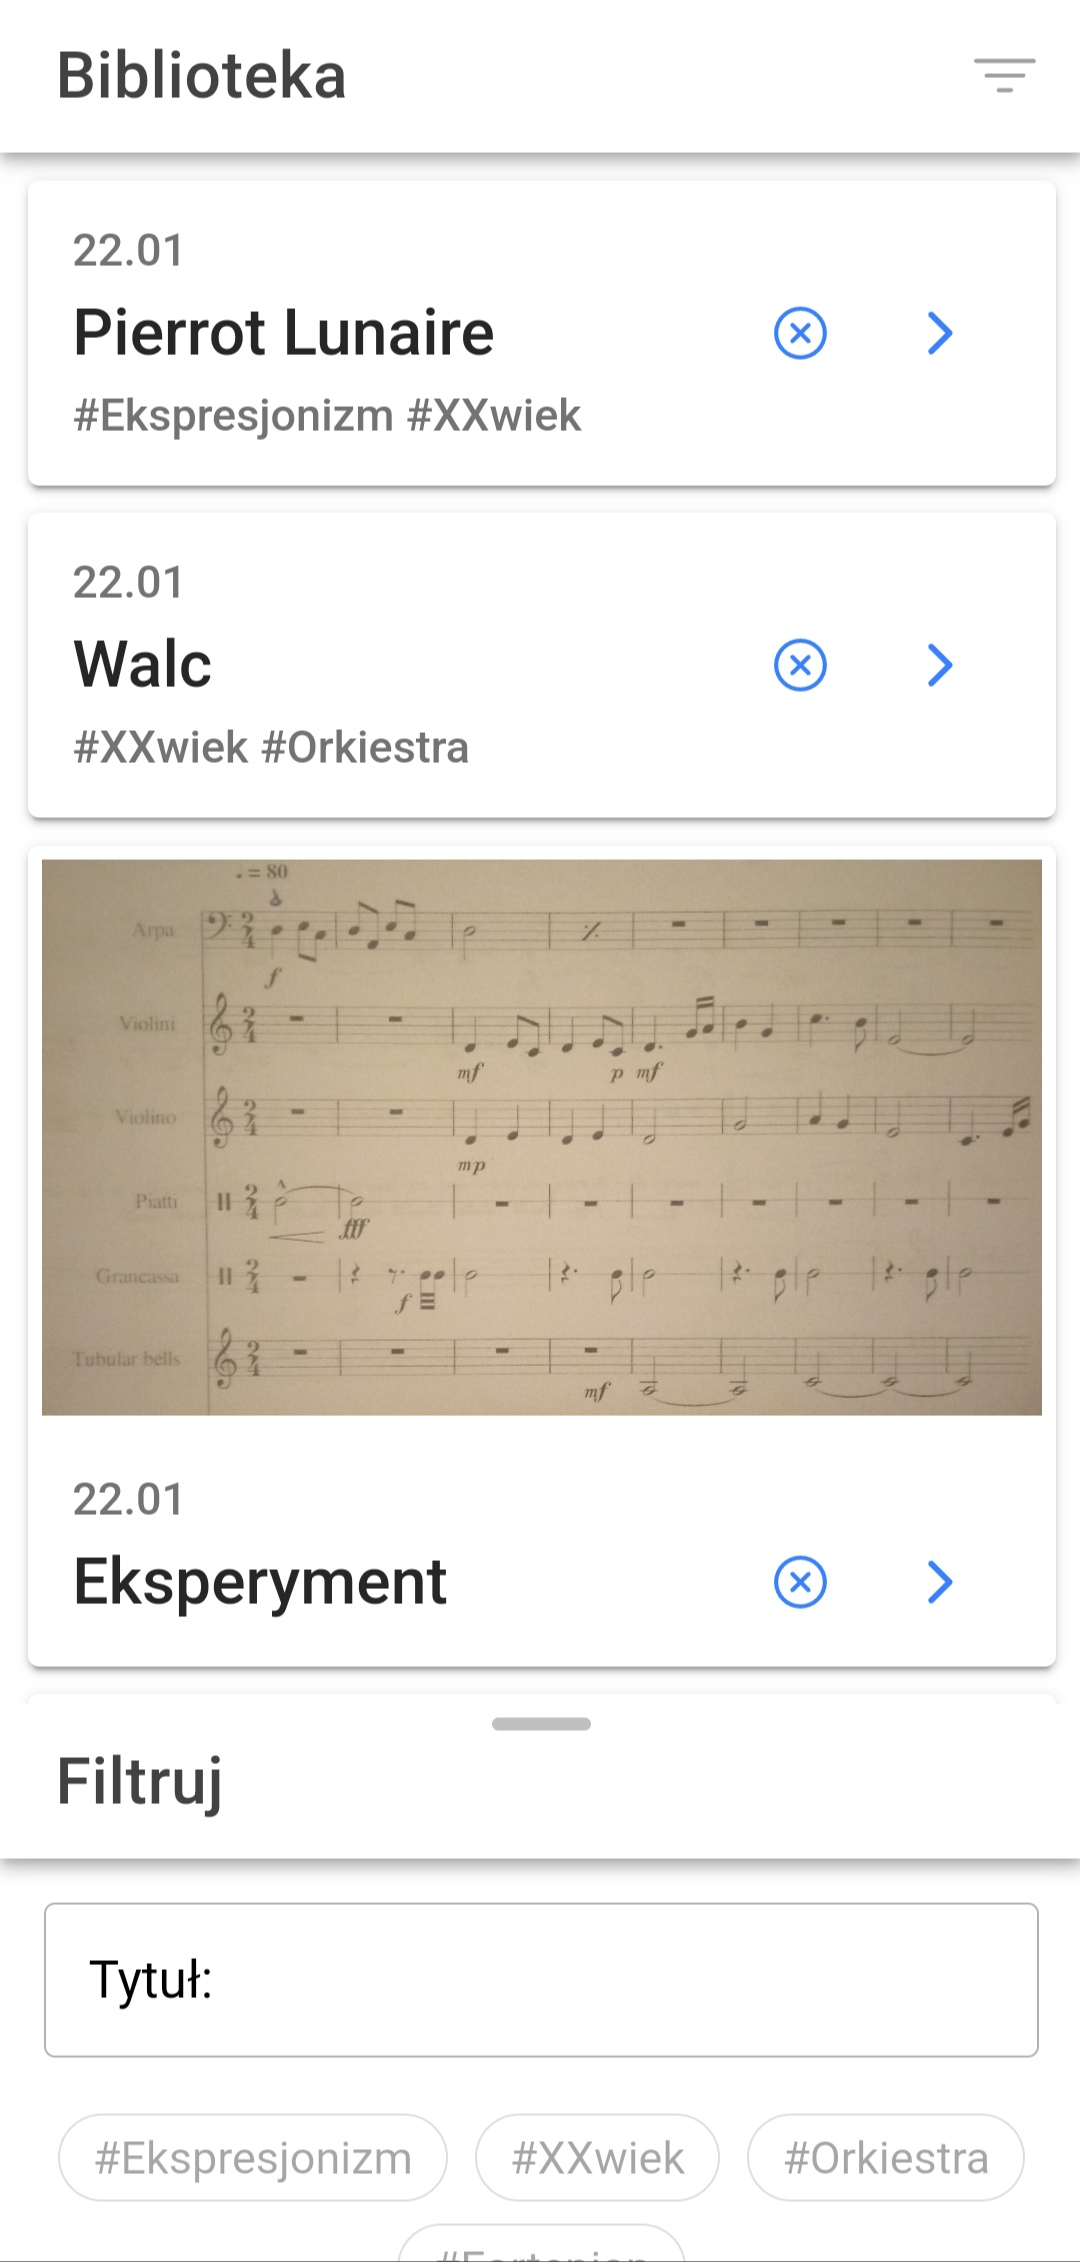
\includegraphics[scale=0.2]{media/LibraryView.jpg}
	\end{center}
	\caption{Widok biblioteki.}
	\label{rys:library-view}
\end{figure}

Możliwość filtracji zeszytów realizowana jest przez modal, otwierany po kliknięciu górnego paska widoku biblioteki.
Użytkownik może przeszukiwać kolekcje po tytułach zeszytów oraz po słowach kluczowych.
Wyszukiwanie po tytule jest case-insensitive.
\begin{figure}[H]
	\begin{center}
		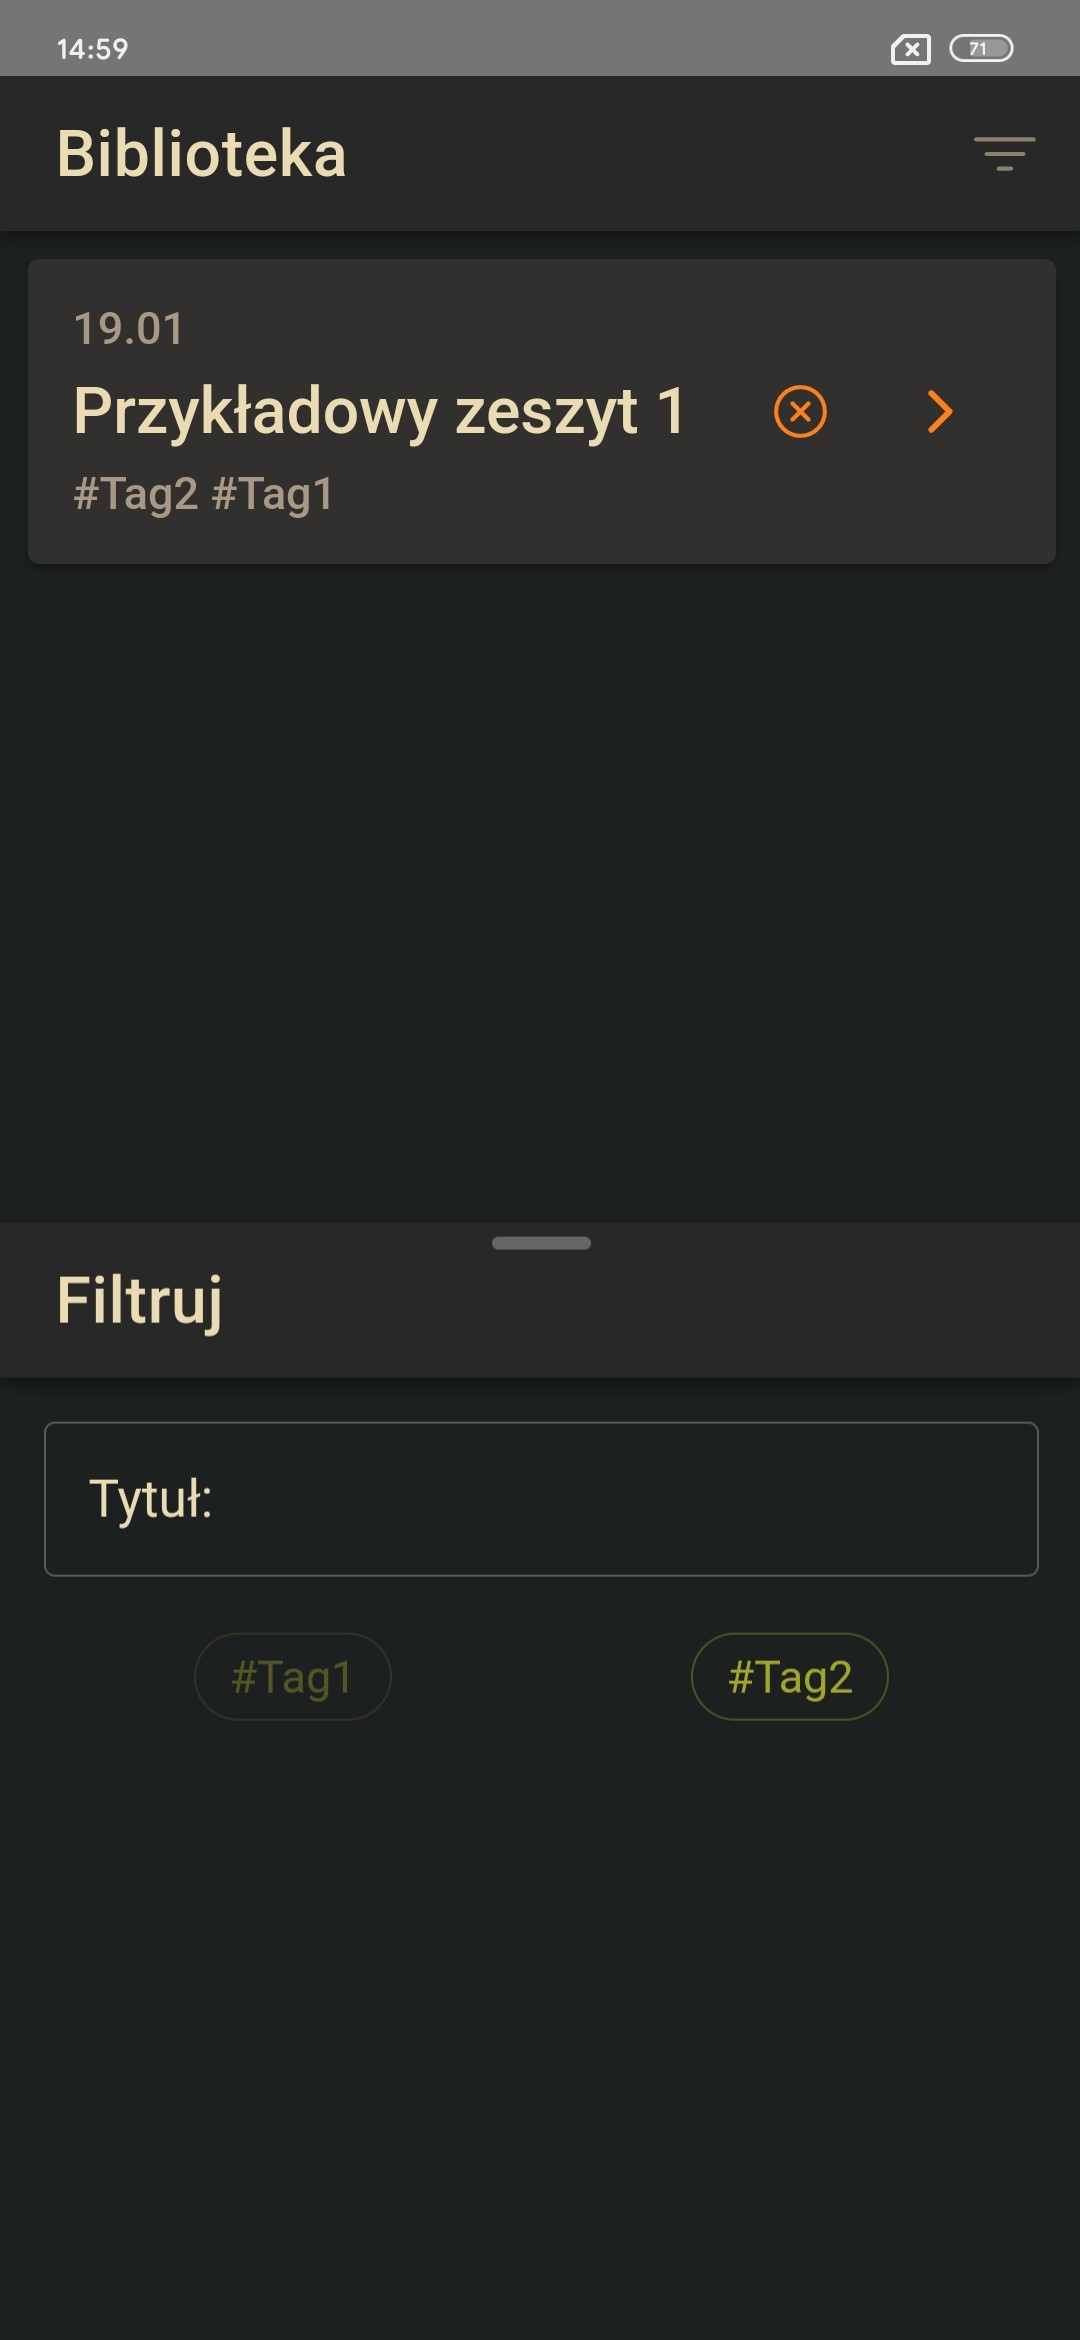
\includegraphics[scale=0.2]{media/FilterModal.jpg}
	\end{center}
	\caption{Modal filtrowania.}
	\label{rys:filter-modal}
\end{figure}

Widok zeszytu umożliwia wizualizację zawartości wybranego zeszytu. Przycisk w rogu ekranu pozwala dodać stronę do zeszytu.
Po dodaniu jest ona reprezentowana przez komponent karty. Zawartość strony może zostać ukryta,
przy użyciu przycisku z symbolem oka. Przytrzymanie przycisku powoduje trwałe usunięcie strony, sygnalizowane wibracją urządzenia.
Strona zawiera także przycisk umożliwiający jej przemieszczenie względem pozostałych stron. W tym miejscu wyświetla się także nazwa
strony, jeżeli została nadana przez użytkownika.
\begin{figure}[H]
	\begin{center}
		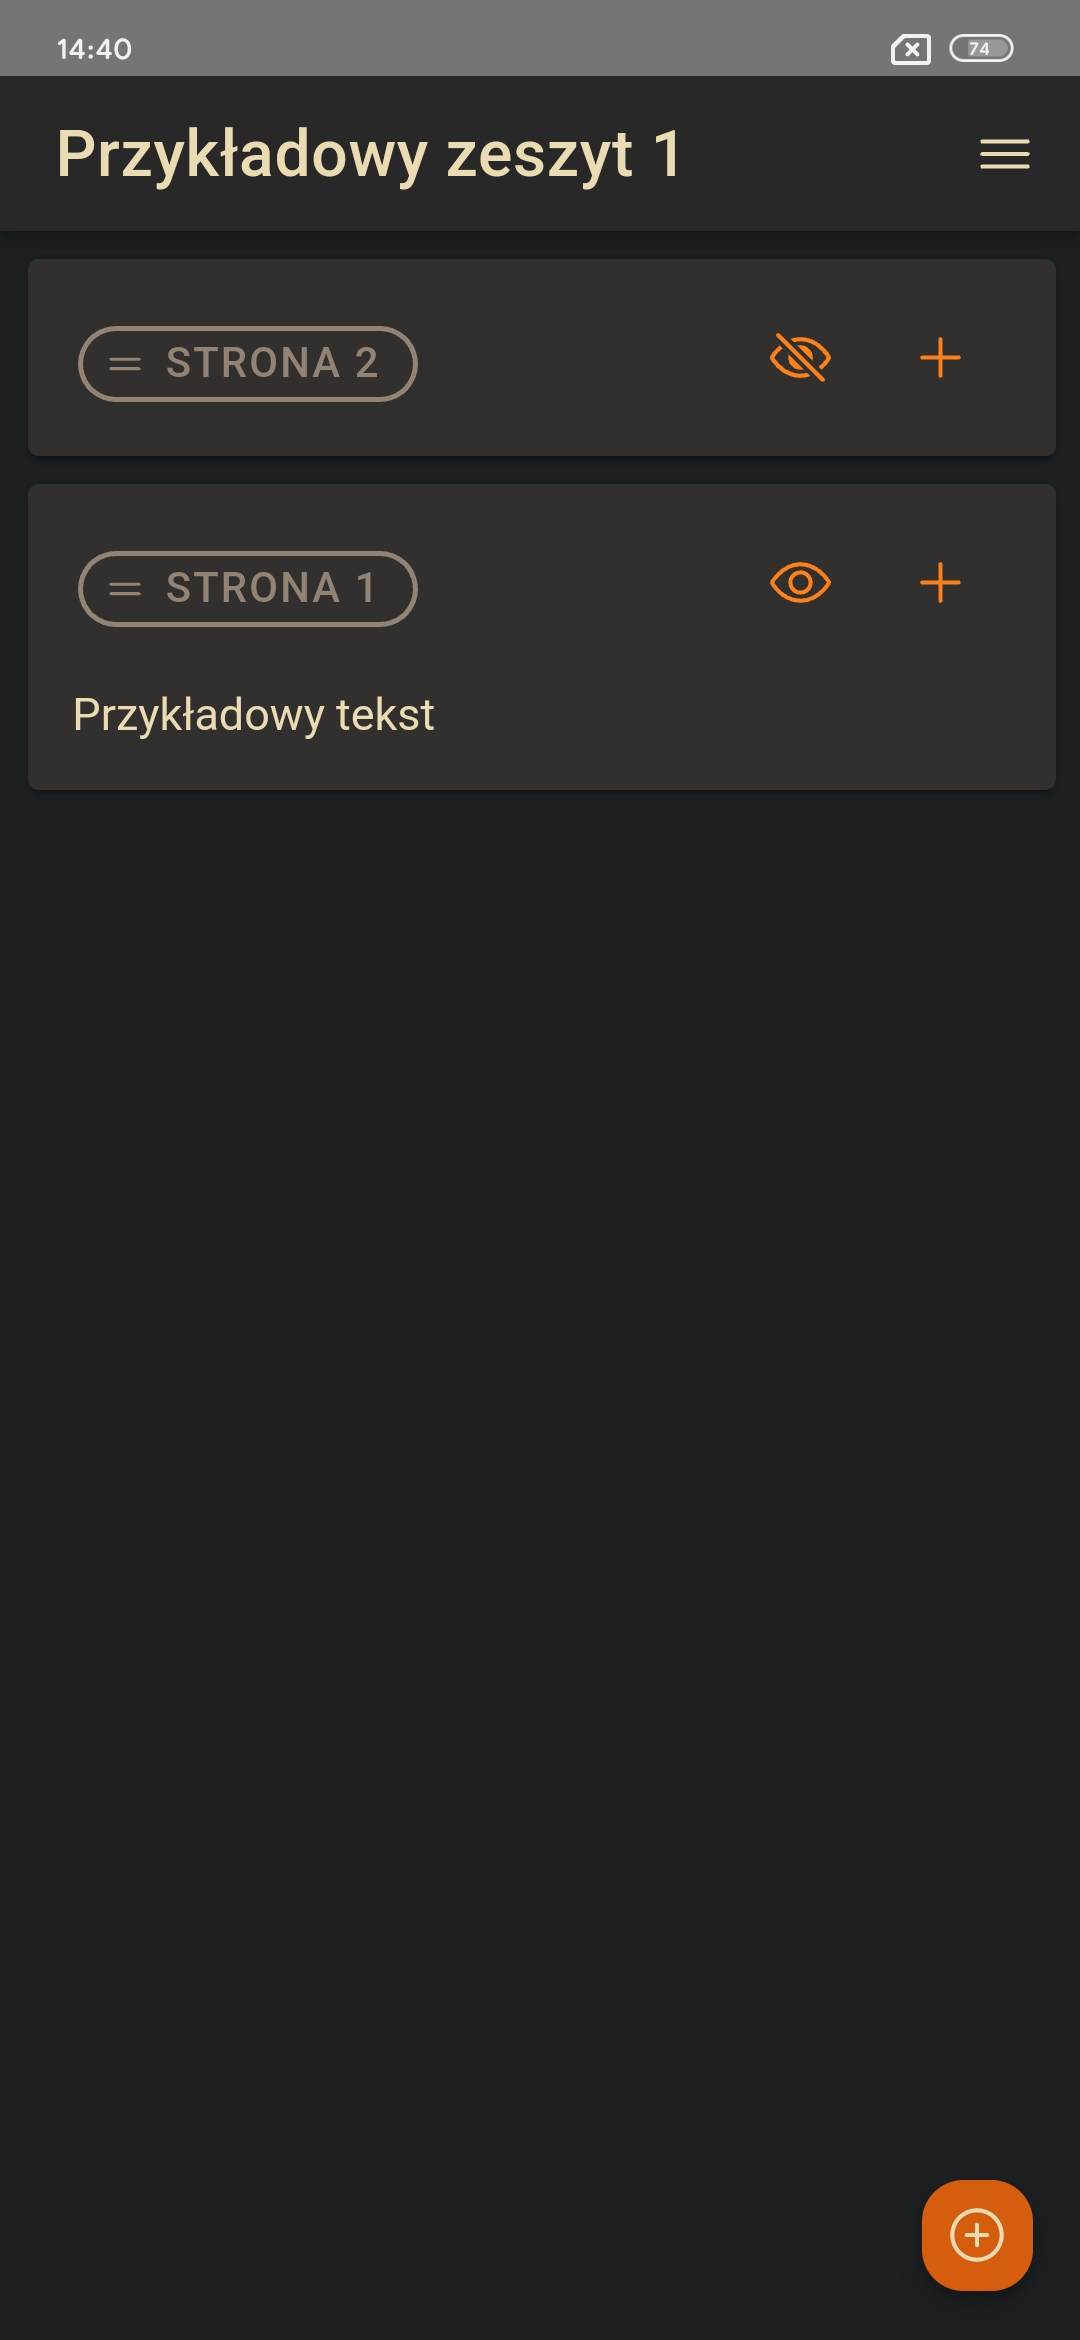
\includegraphics[scale=0.2]{media/BookView.jpg}
	\end{center}
	\caption{Widok zeszytu.}
	\label{rys:book-view}
\end{figure}

Możliwość edycji strony realizowana jest przez modal, otwierany po kliknięciu ikony plusa. Zawartość modalu zależy od
typu edytowanej strony, umożliwiając stosowny interfejs edycji zawartości. Każdej stronie można tu również przypisać nazwę.
\begin{figure}[H]
	\begin{center}
		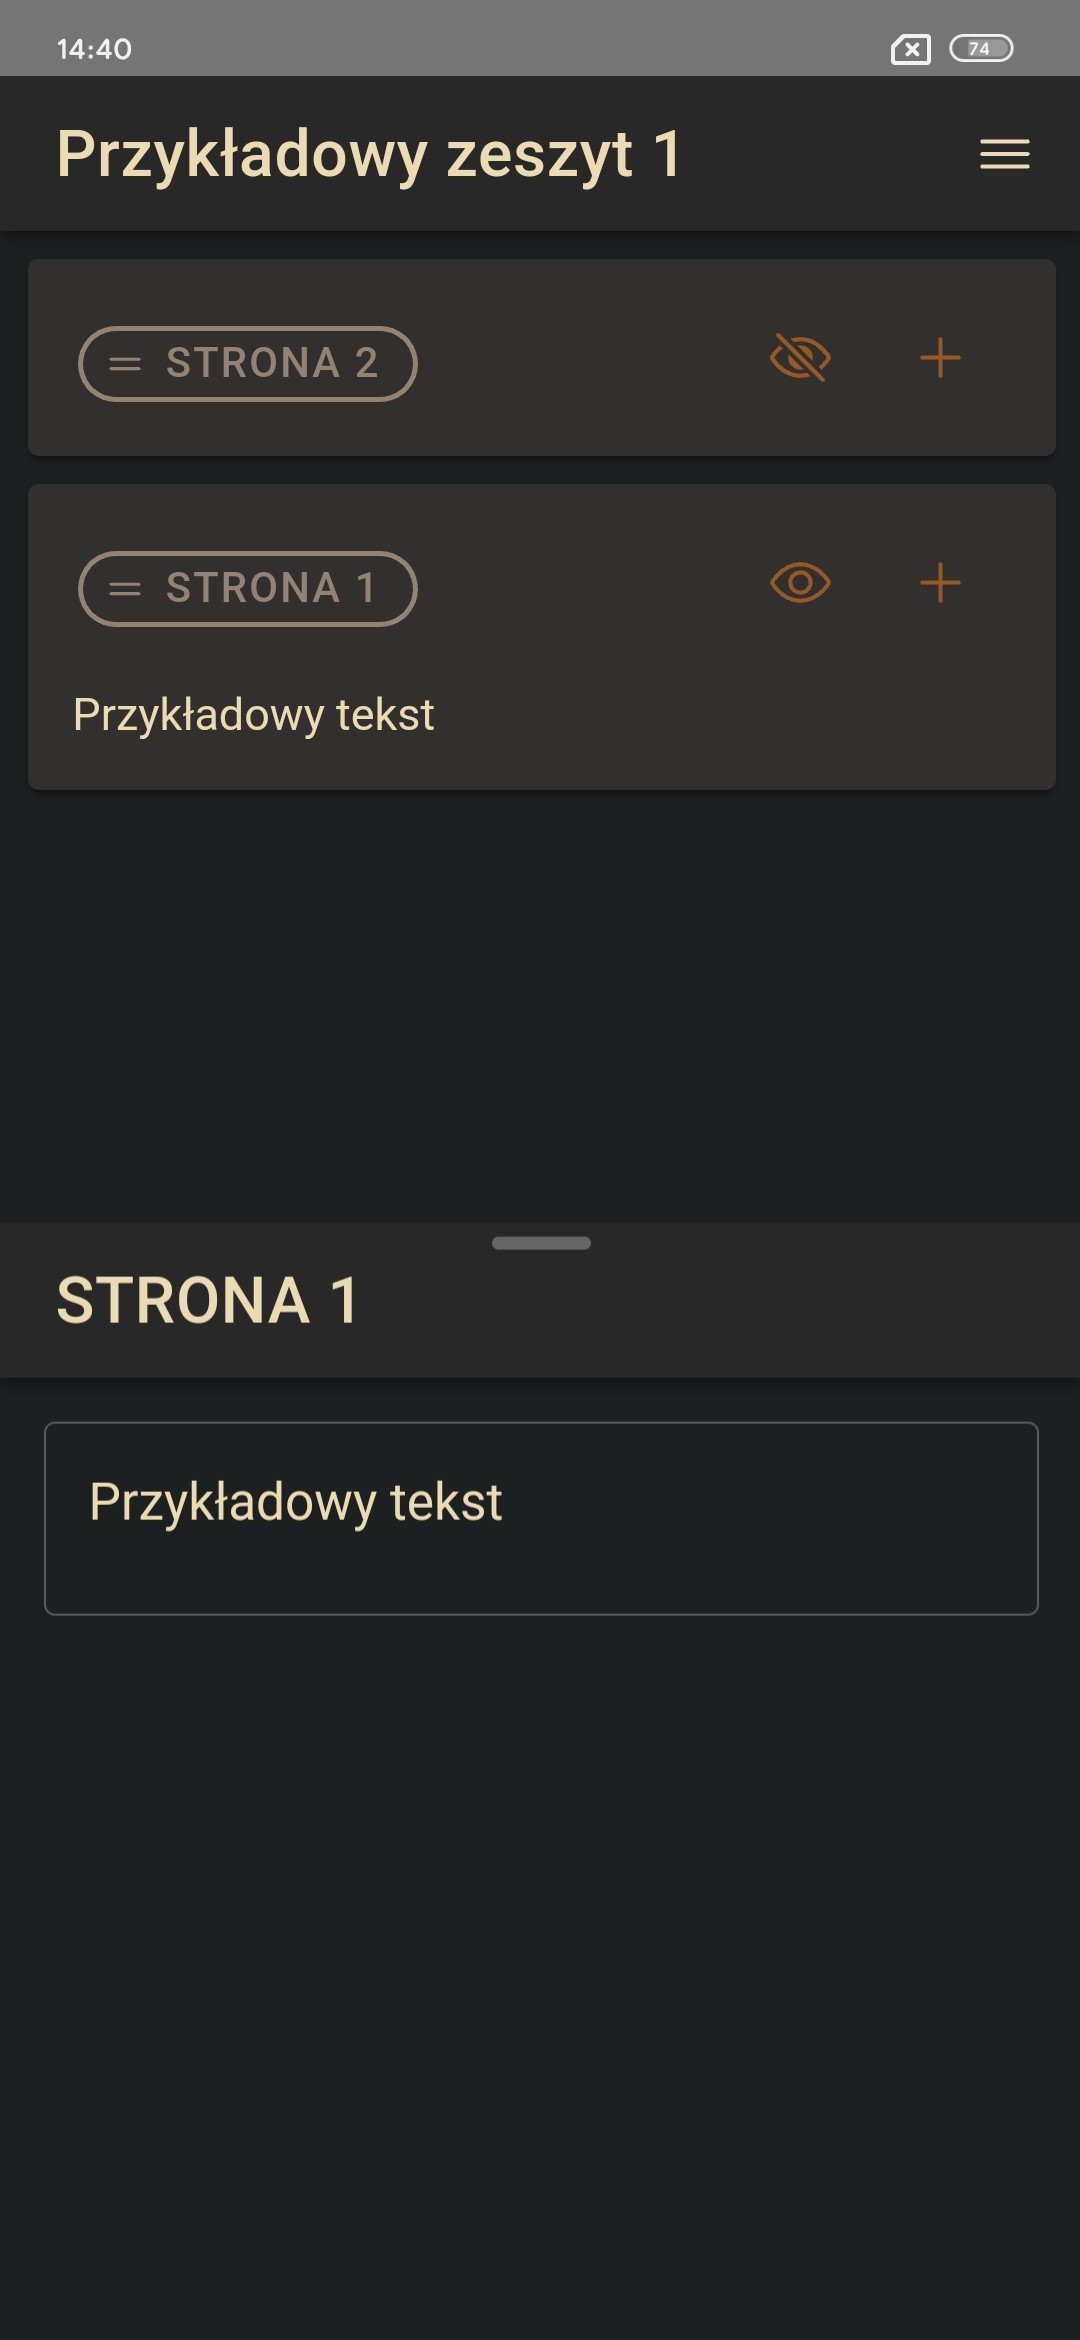
\includegraphics[scale=0.2]{media/EditorModal.jpg}
	\end{center}
	\caption{Modal edycji strony.}
	\label{rys:editor-modal}
\end{figure}

Modyfikacja danych zeszytu umożliwiana jest przez menu, otwierane przy kliknięciu górnego paska widoku zeszytu.
Przycisk z ikoną zdjęcia umożliwia dodanie okładki; kliknięcie symbolu zakładki pozwala przypisać słowo kluczowe
do zeszytu. Można w tym miejscu również zmienić tytuł zeszytu.
\begin{figure}[H]
	\begin{center}
		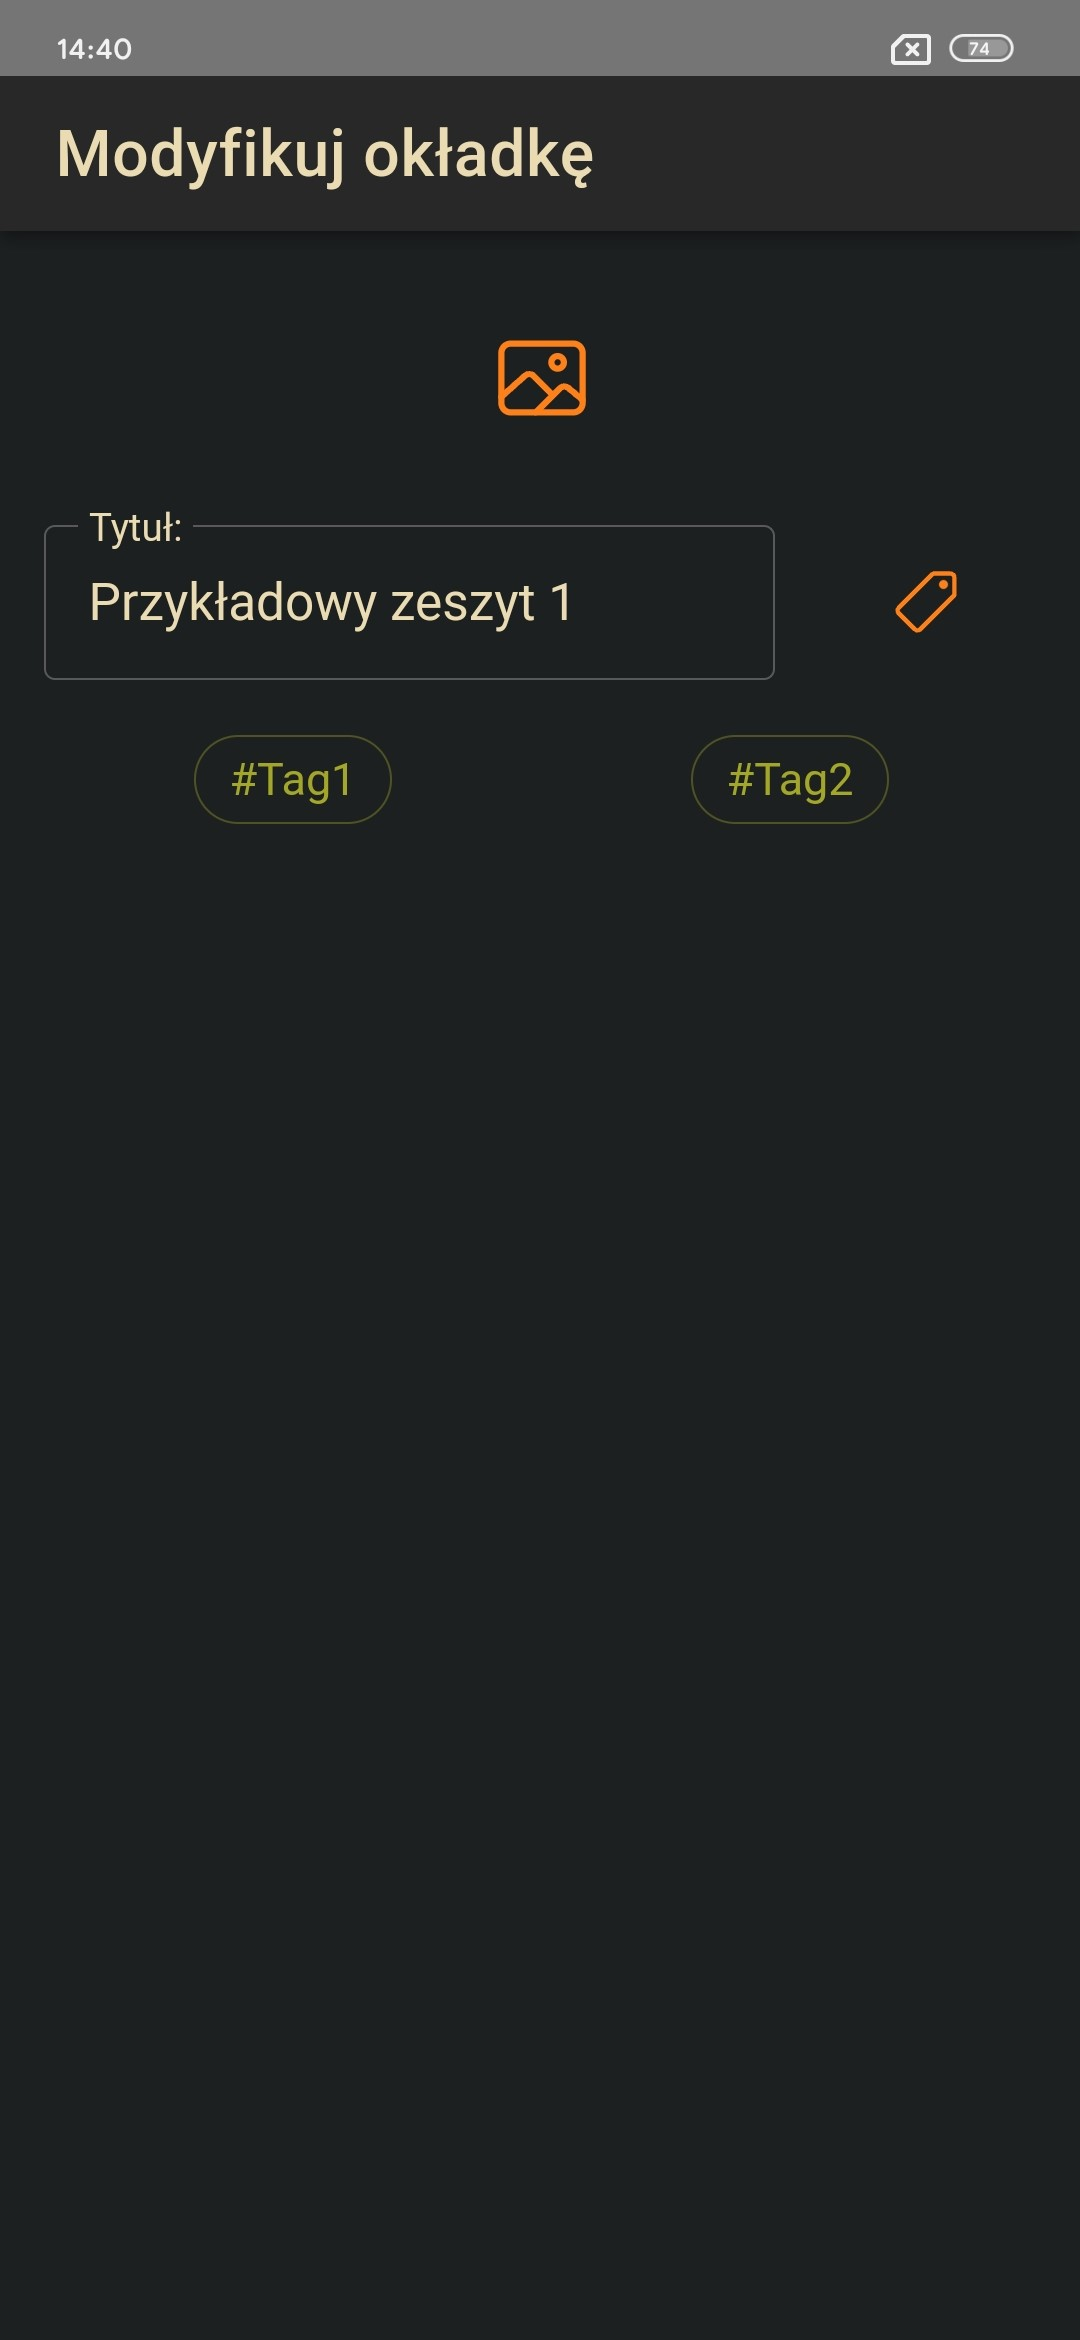
\includegraphics[scale=0.2]{media/BookMenu.jpg}
	\end{center}
	\caption{Menu edycji danych zeszytu.}
	\label{rys:book-menu}
\end{figure}

\subsubsection{Implementacja funkcjonalności wspierających aranżację}
Przedstawione wcześniej komponenty stanowią \enquote{środowisko}, które umożliwiaja implementację konkretnych funkcjonalności
wspierających proces aranżacji muzycznej. Realizowane są one przez podział stron na cztery zdefiniowane typy.
Charakteryzują się one odmiennym rodzajem wizualizacji oraz zróżnicowanym procesem edycji. Aby to umożliwić, komponenty główne
dopasowują dynamicznie komponenty odpowiadające za wizualizację i edycję stron w zależności od ich typu.
Dynamiczne dopasowanie jest realizowane dzięki zastosowaniu \textit{component-is} oferowanego przez Vue.

Komponenty wizualizacji i edycji tekstu obsługują notatki tekstowe, umożliwiając dodawanie subtelnych (jako: nieodwracających uwagi)
komentarzy. Podczas edycji użytkownik zapisuje notatkę w polu tekstowym. Linijka tekstu poprzedzona symbolem \enquote{@} traktowana jest
jako komentarz. Aby to ułatwić, układ klawiatury przy edycji treści takiej strony ustawiony jest na tryb \textit{e-mail}.
Komentarz wyświetlany jest przy prawej krawędzi strony, mniej wyrazistą czcionką.
\begin{figure}[H]
	\begin{center}
		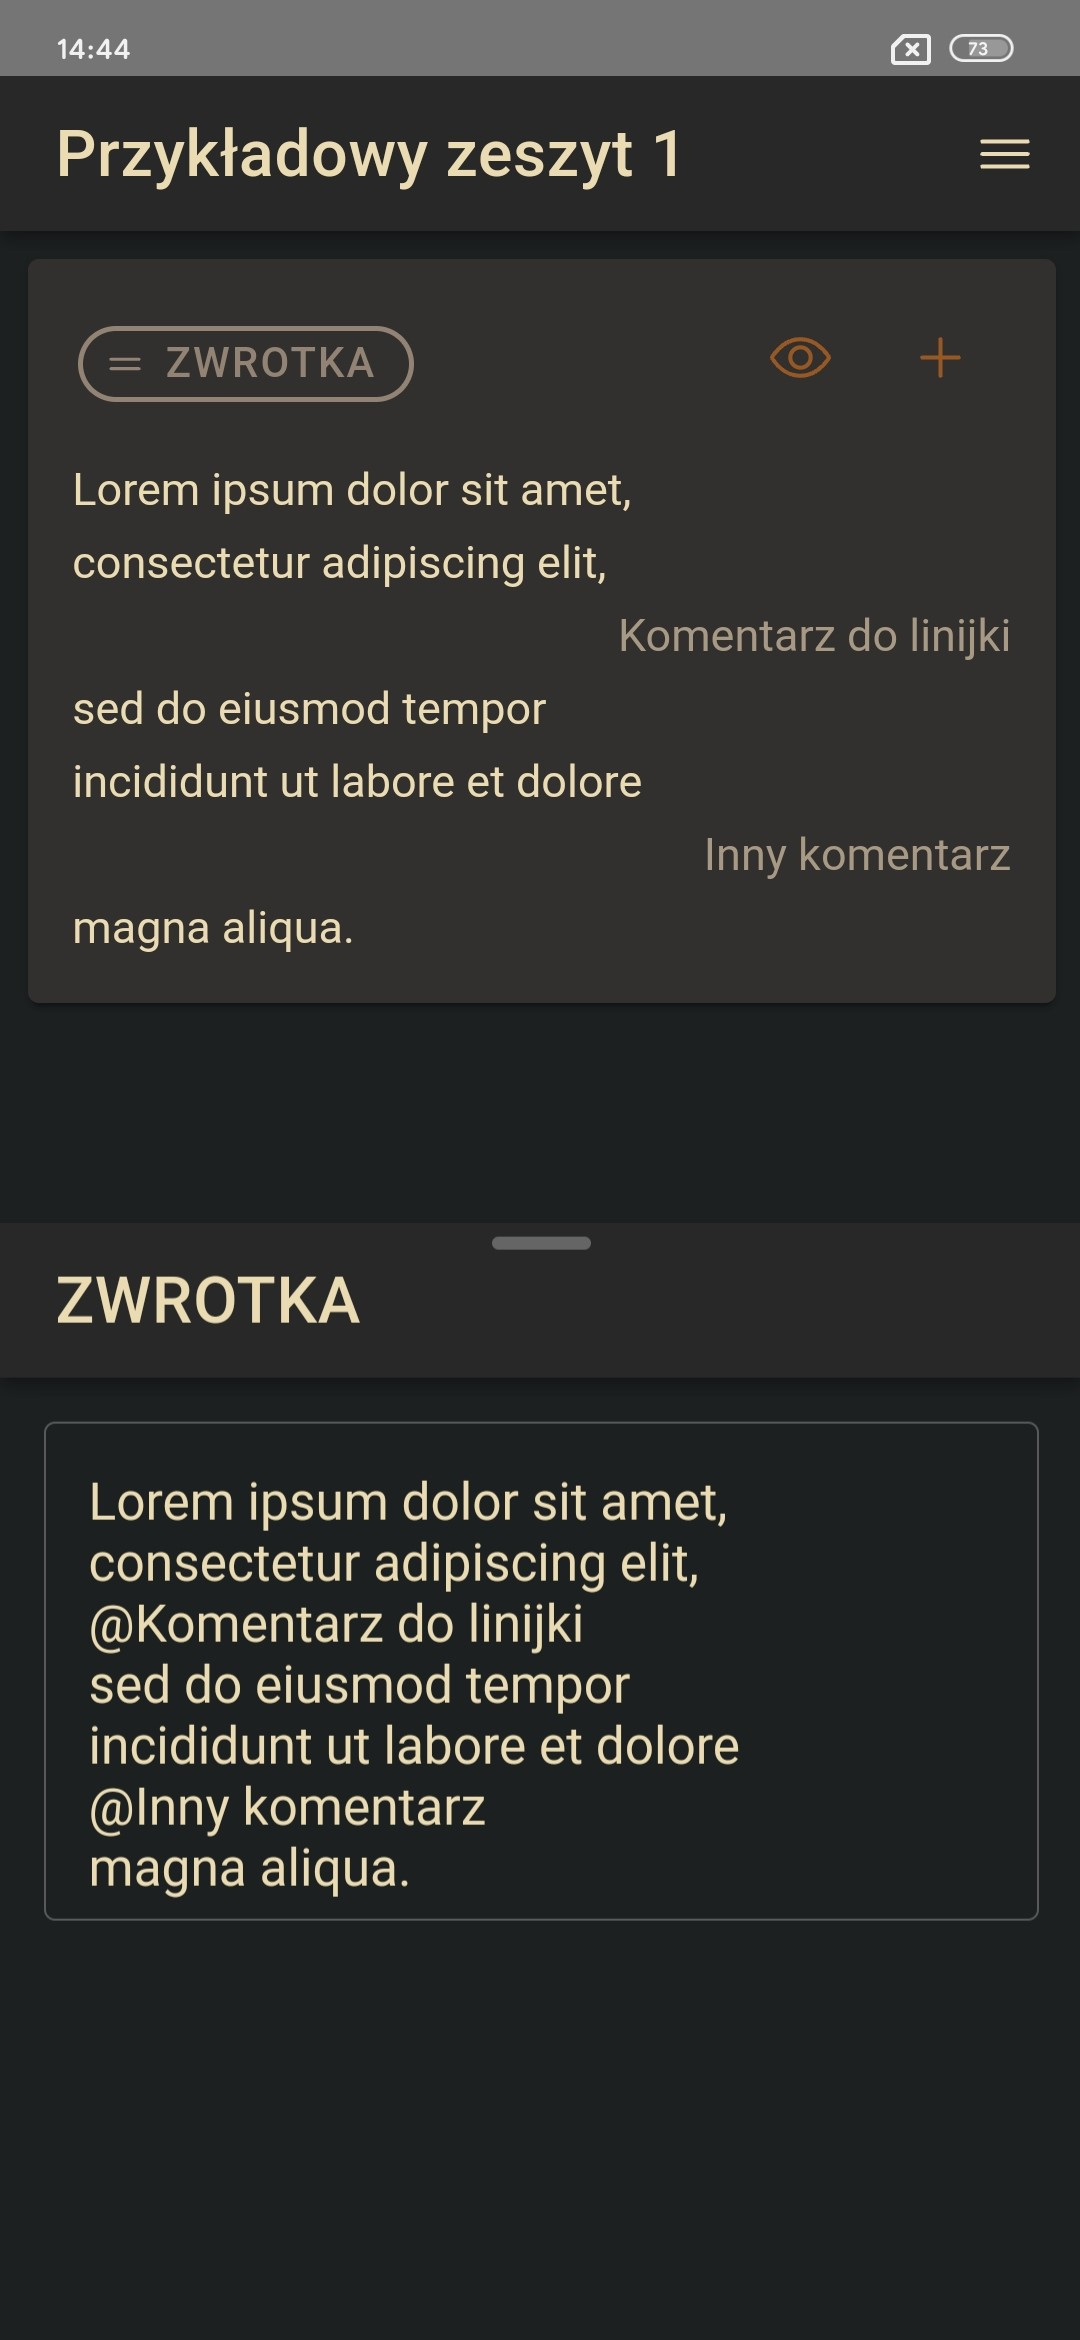
\includegraphics[scale=0.2]{media/TextPage.jpg}
	\end{center}
	\caption{Komponenty strony o typie tekstowym.}
	\label{rys:text-page}
\end{figure}

Wizualizacja zapisu nutowego realizowana jest przy użyciu biblioteki ABC.js. W ramach komponentu umożliwiającego edycję
użytkownik znów zapisuje notatkę w polu tekstowym, lecz jest ona renderowana jako zapis nutowy w komponencie strony. Pomocna jest tu forma komponentu modala,
jako umożliwiającego śledzenie zmian zapisu nutowego podczas jego edycji. Z uwagi na przystępną zasadę działania biblioteki
ABC.js — za sprawą stosowania nazw literowych do określania nut, nie jest wymagane stosowanie edytorów.
Każda taka strona domyślnie inicjalizowana jest wartościami renderującymi kluczowe elementy notacji muzycznej.
Jednocześnie należy zwrócić uwagę, że użytkownik potrzebujący szerszych możliwości edytora nutowego, powinien zaznajomić
się z dodatkowymi funkcjami oferowanymi przez ABC.js.
\begin{figure}[H]
	\begin{center}
		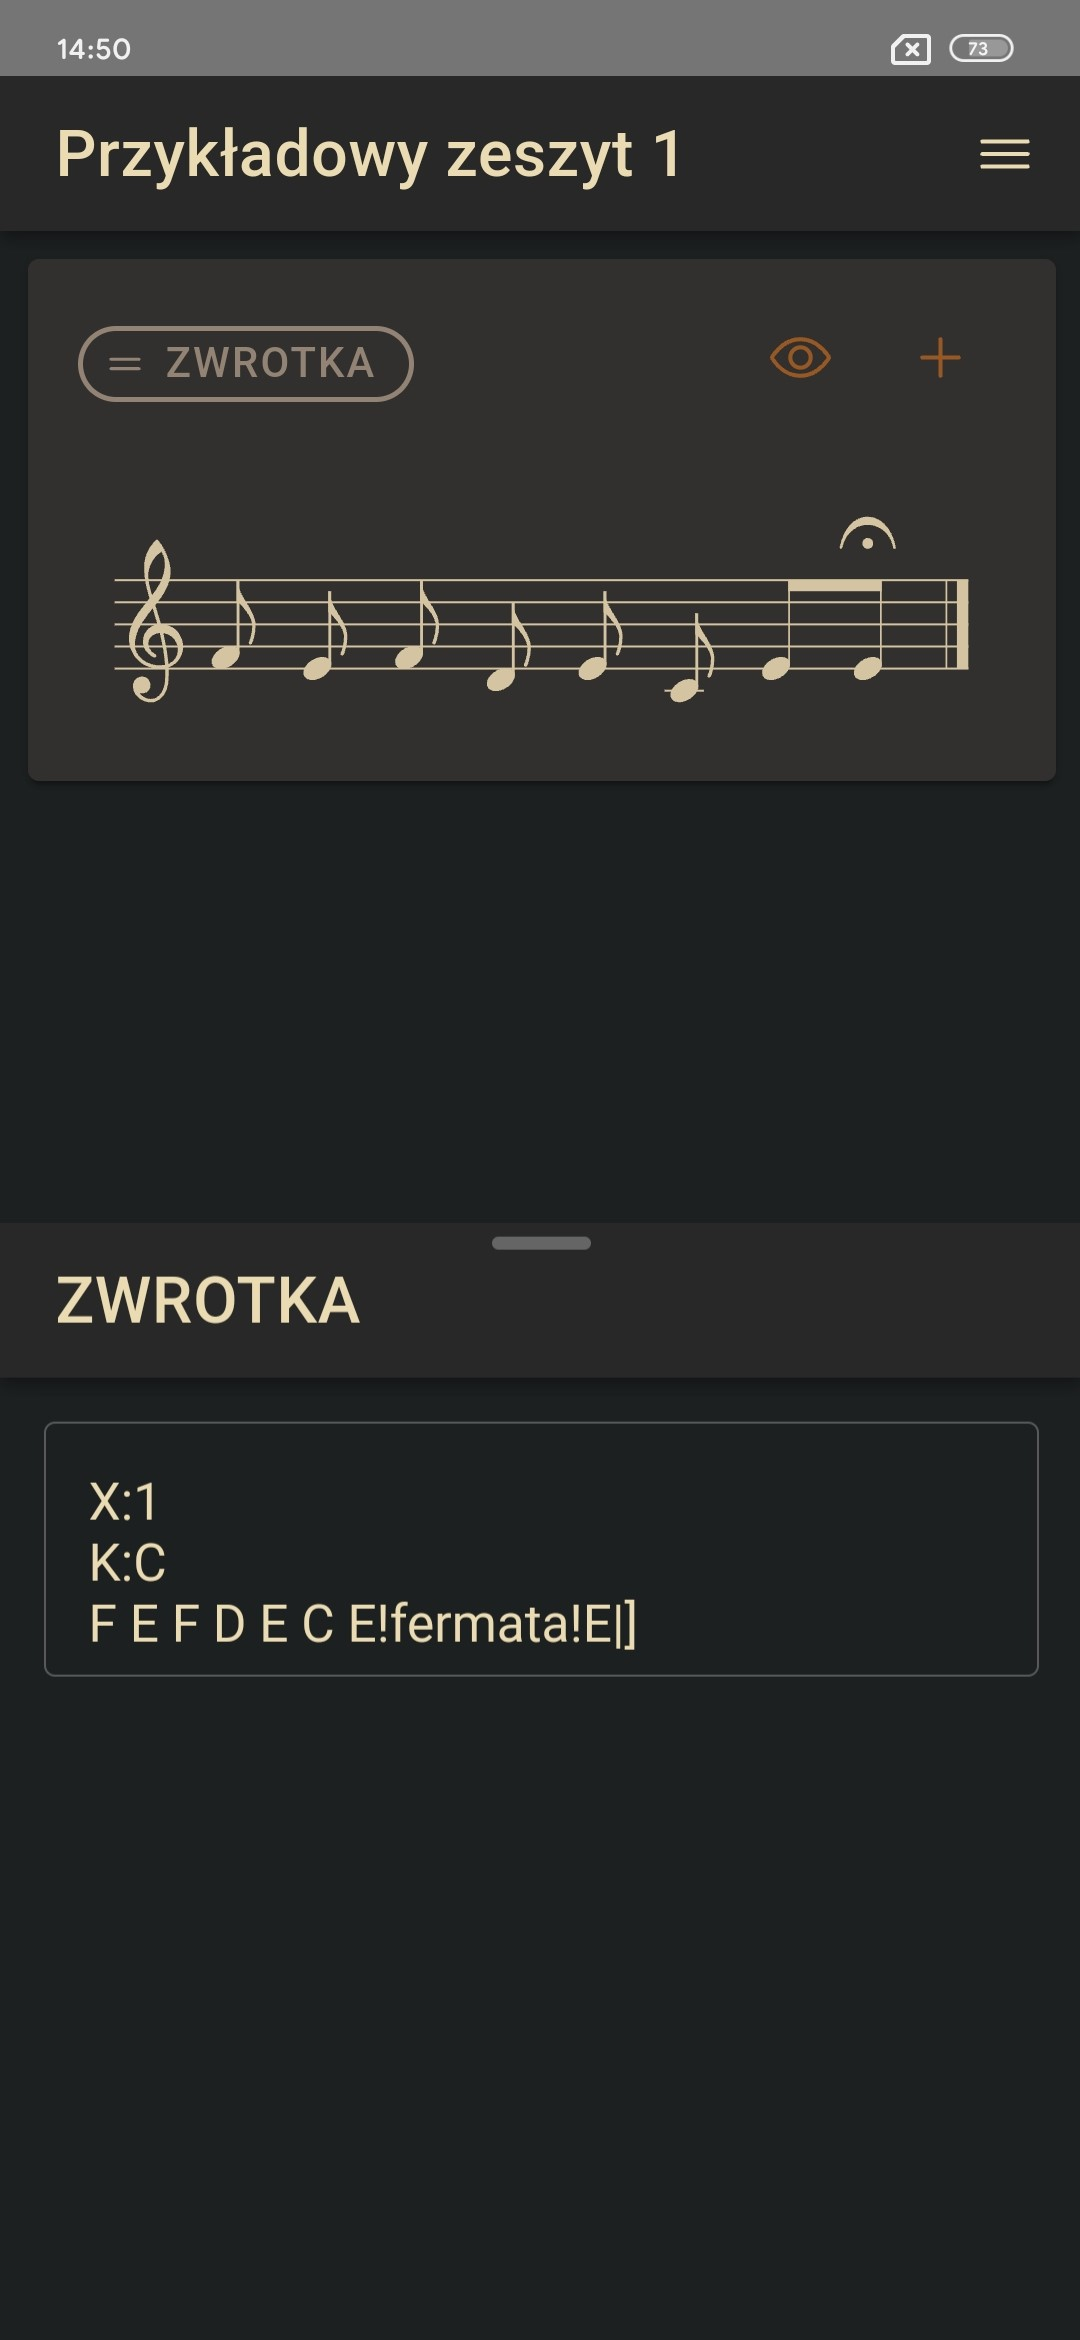
\includegraphics[scale=0.2]{media/ScorePage.jpg}
	\end{center}
	\caption{Komponenty strony o typie nutowym.}
	\label{rys:score-page}
\end{figure}

Komponent edycji notatek dźwiękowych wykorzystuje do działania wtyczkę capacitor-voice-recorder. Pozwala ona nagrać
dźwięk, korzystając z mikrofonu urządzenia. Po nagraniu użytkonik może ponownie edytować zawartość strony, zastępując
wcześniejszy zapis dźwiękowy nowym nagraniem. Wizualizacja fali dźwiękowej, realizowana przez bibliotekę Wavesurfer.js,
umożliwia orientację w jej przebiegu oraz odtworzenie nagrania od wybranego momentu.
\begin{figure}[H]
	\begin{center}
		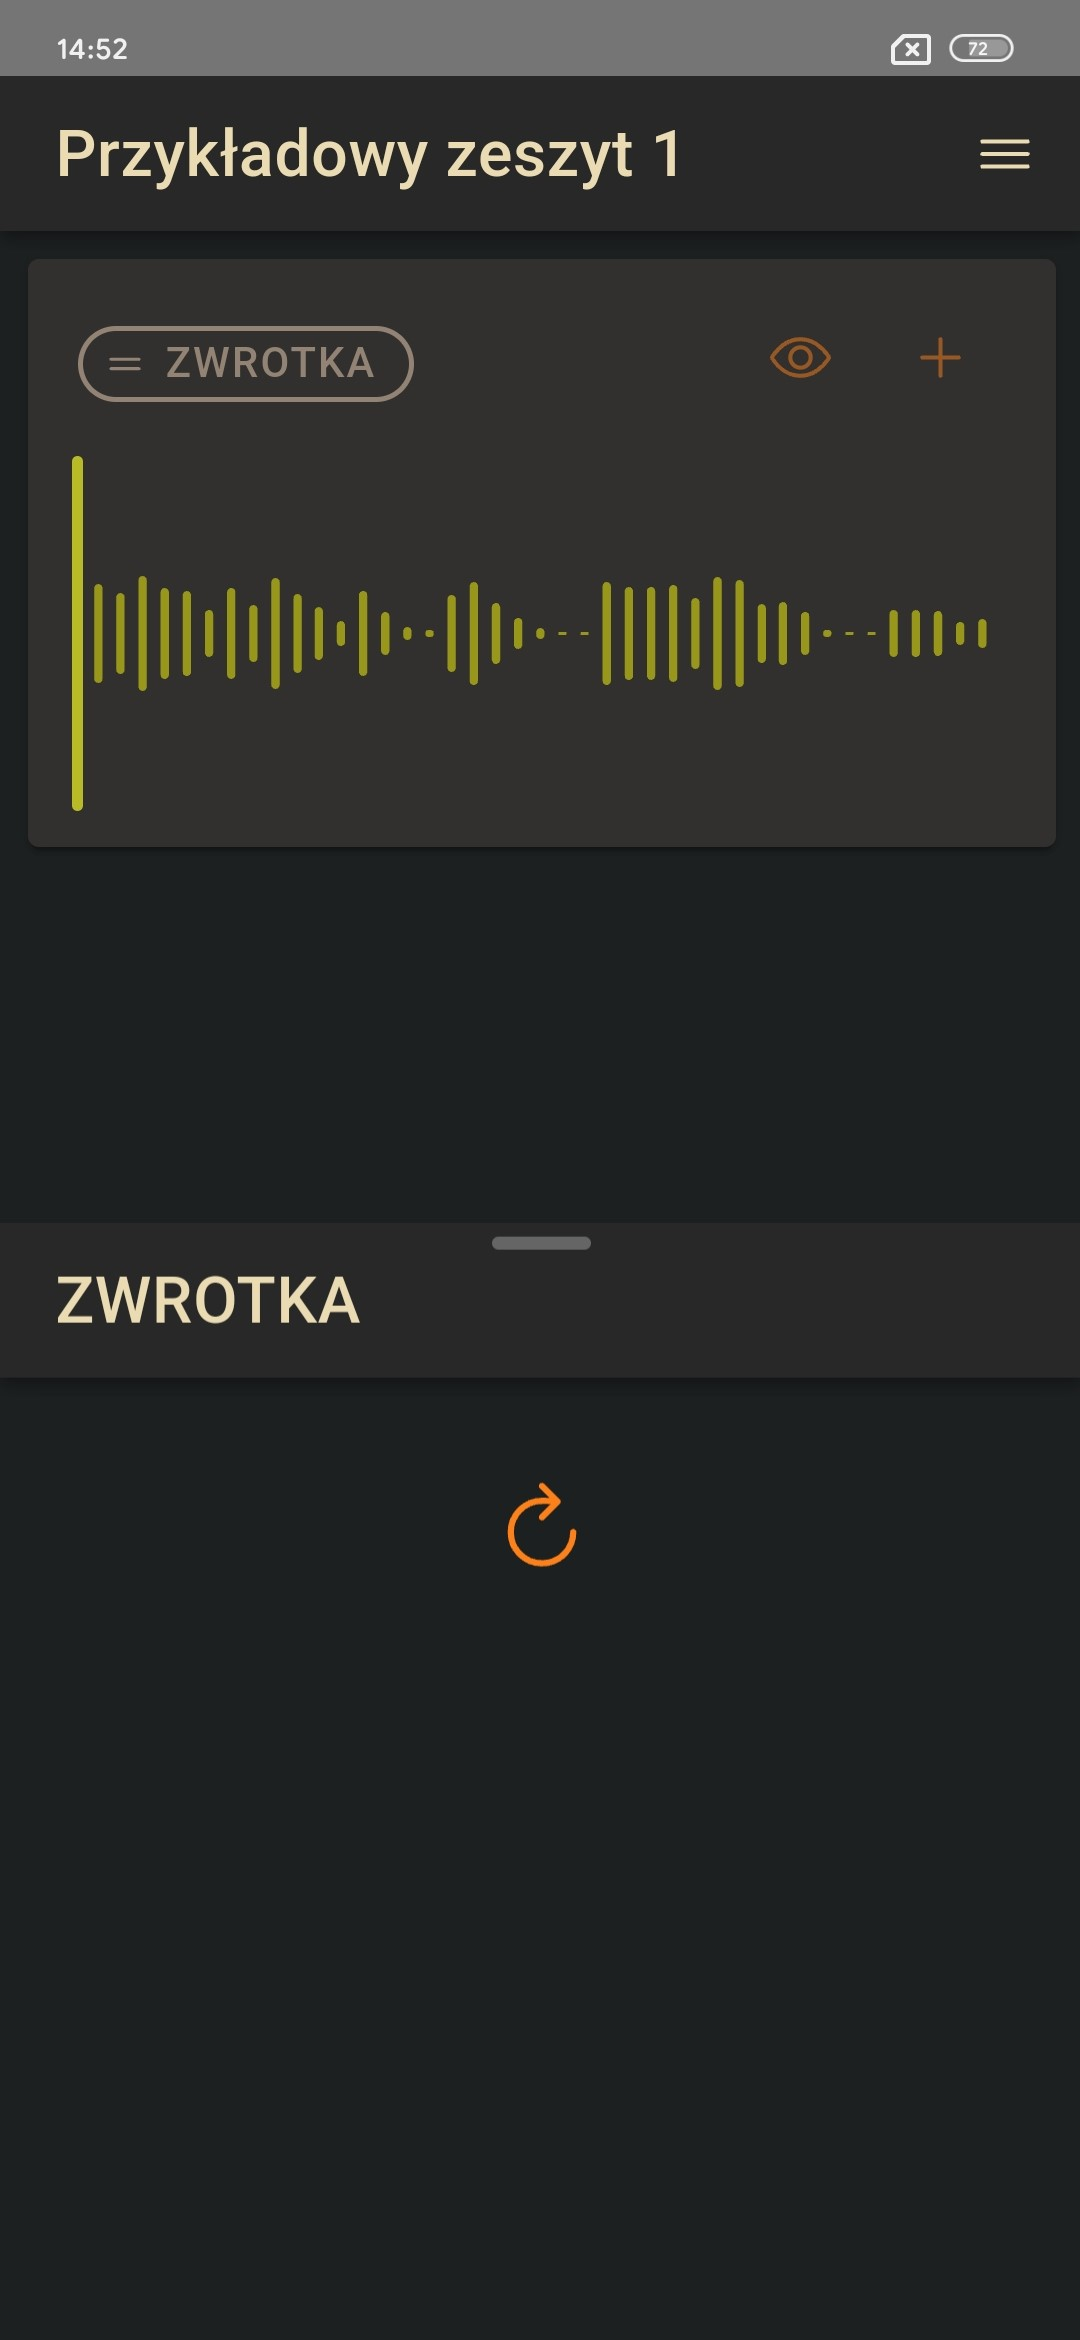
\includegraphics[scale=0.2]{media/AudioPage.jpg}
	\end{center}
	\caption{Komponenty strony zawierającym nagranie audio.}
	\label{rys:audio-page}
\end{figure}

Możliwość dołączenia zdjęcia jako notatki realizowana jest przy zastosowaniu wtyczki capacitor-file-picket,
pozwalającej wybrać plik (tu: zdjęcie) z pamięci urządzenia. Wybrane zdjęcie jest wyświetlane jako zawartość strony.
Edycja strony polega na możliwości zmiany wybranego zdjęcia na inne.
\begin{figure}[H]
	\begin{center}
		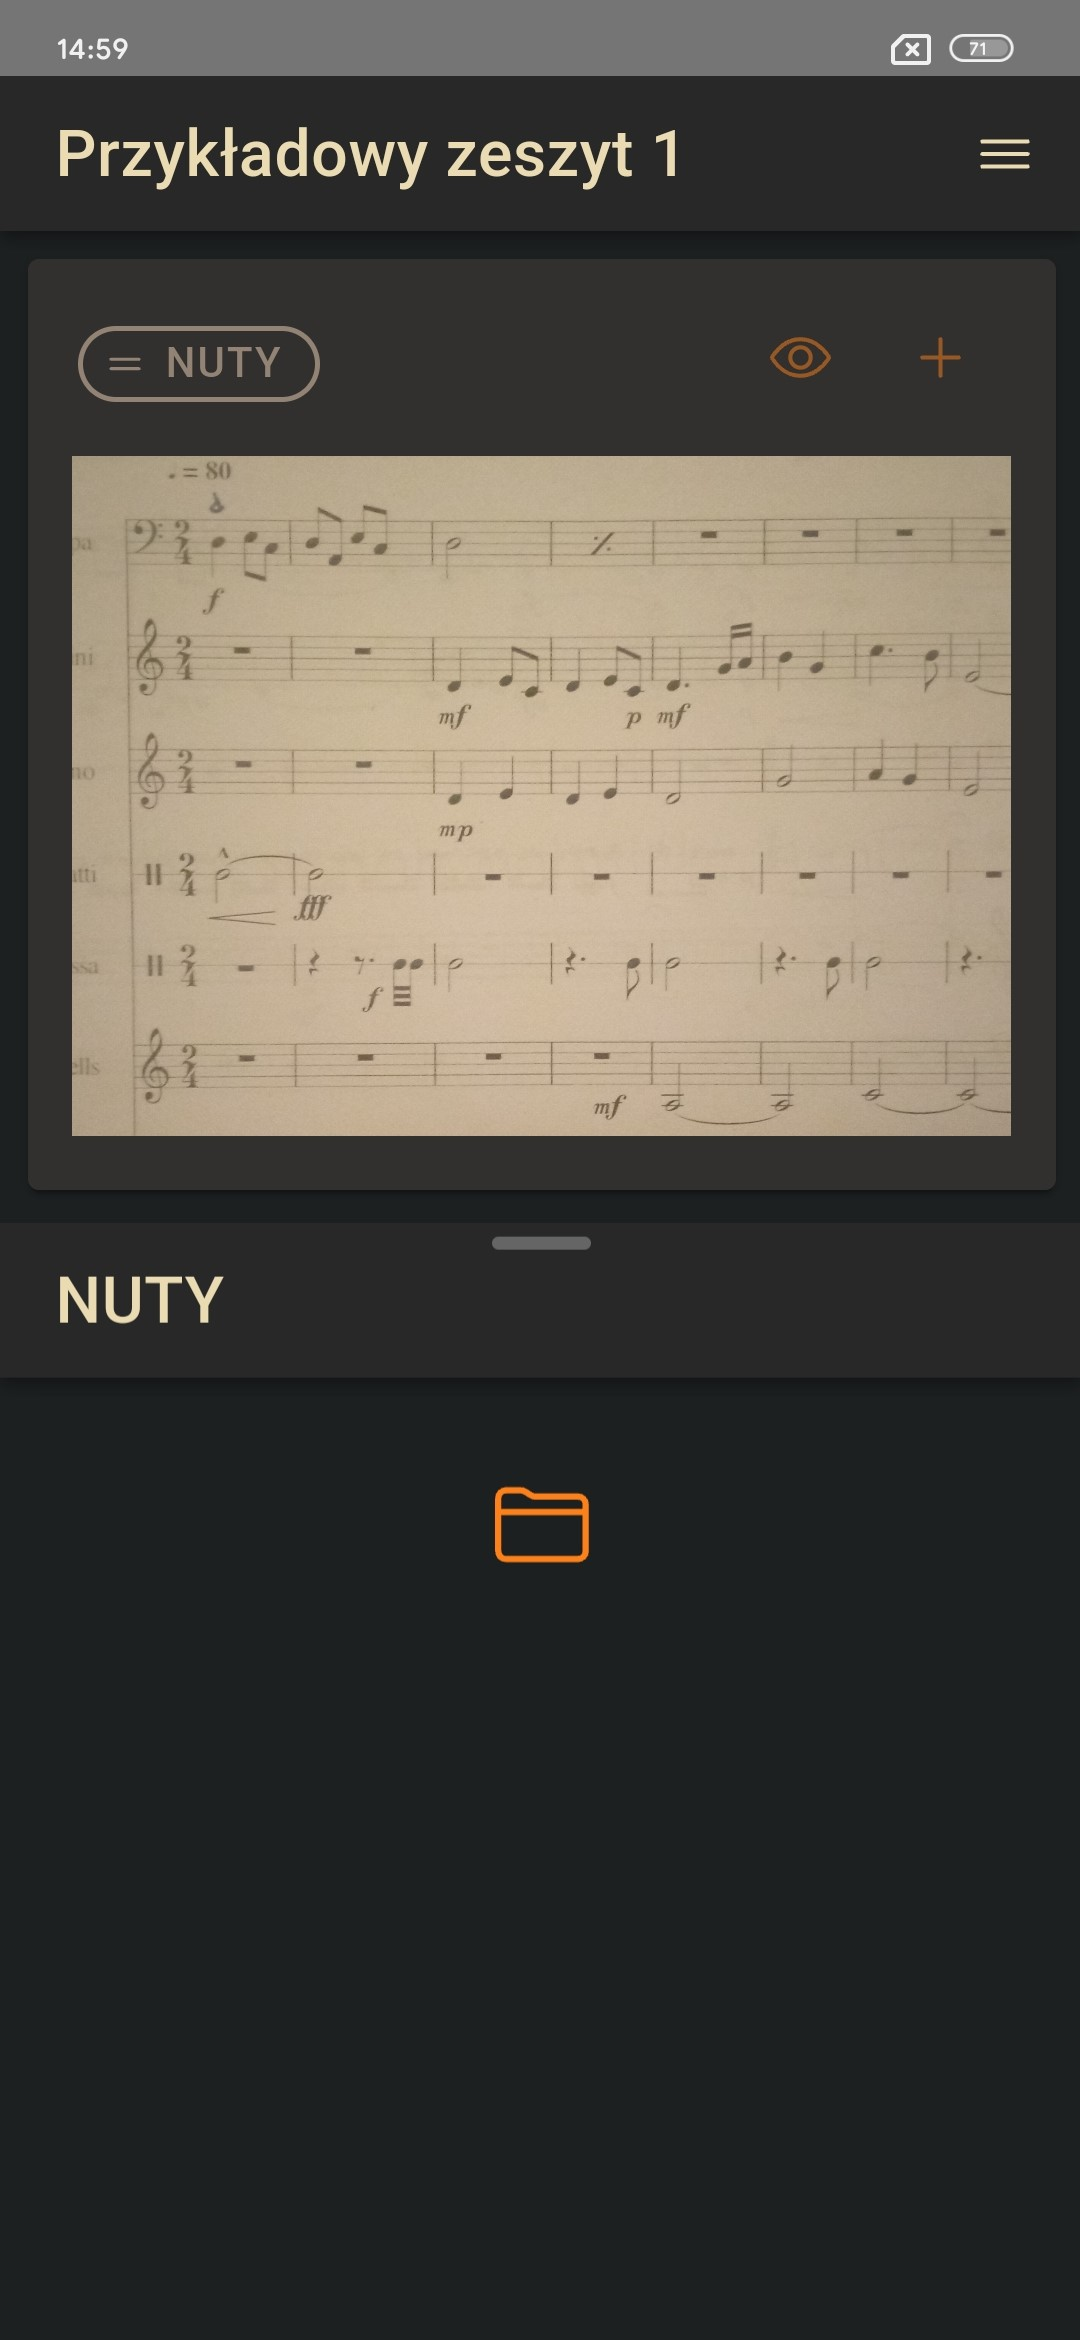
\includegraphics[scale=0.2]{media/PhotoPage.jpg}
	\end{center}
	\caption{Komponenty strony zawierającej zdjęcie.}
	\label{rys:photo-page}
\end{figure}

\subsection{Testowanie aplikacji}

opisać implementacje
drzewo komponentów
